
%<<setup-child, include = FALSE>>=

%library(knitr)
%options(digits = 16)

%library(RCurl)
%library(XML)
%library(tm)
%library(NMF)
%library(microbenchmark)
%library(ggplot2)
%library(wordcloud)
%set_parent("../style/preamble.Rnw")
%@


\newcommand{\xdownarrow}[1]{%
	{\left\downarrow\vbox to #1{}\right.\kern-\nulldelimiterspace}
}

\newcommand{\grey}[1]{\textcolor{grey}{#1}}
\newcommand{\red}[1]{\textcolor{red}{#1}}

\input{../../2021/style/preamble4tex}
% dependencies: amsmath, amssymb, dsfont
% math spaces
\ifdefined\N
\renewcommand{\N}{\mathds{N}} % N, naturals
\else \newcommand{\N}{\mathds{N}} \fi
\newcommand{\Z}{\mathds{Z}} % Z, integers
\newcommand{\Q}{\mathds{Q}} % Q, rationals
\newcommand{\R}{\mathds{R}} % R, reals
\ifdefined\C
\renewcommand{\C}{\mathds{C}} % C, complex
\else \newcommand{\C}{\mathds{C}} \fi
\newcommand{\continuous}{\mathcal{C}} % C, space of continuous functions
\newcommand{\M}{\mathcal{M}} % machine numbers
\newcommand{\epsm}{\epsilon_m} % maximum error

% counting / finite sets
\newcommand{\setzo}{\{0, 1\}} % set 0, 1
\newcommand{\setmp}{\{-1, +1\}} % set -1, 1
\newcommand{\unitint}{[0, 1]} % unit interval

% basic math stuff
\newcommand{\xt}{\tilde x} % x tilde
\newcommand{\argmin}{\mathop{\mathrm{arg\,min}}} % argmin
\newcommand{\argmax}{\mathop{\mathrm{arg\,max}}} % argmax
\newcommand{\argminlim}{\argmin\limits} % argmin with limits
\newcommand{\argmaxlim}{\argmax\limits} % argmax with limits
\newcommand{\sign}{\operatorname{sign}} % sign, signum
\newcommand{\I}{\mathbb{I}} % I, indicator
\newcommand{\order}{\mathcal{O}} % O, order
\newcommand{\bigO}{\mathcal{O}} % Big-O Landau
\newcommand{\littleo}{{o}} % Little-o Landau
\newcommand{\pd}[2]{\frac{\partial{#1}}{\partial #2}} % partial derivative
\newcommand{\floorlr}[1]{\left\lfloor #1 \right\rfloor} % floor
\newcommand{\ceillr}[1]{\left\lceil #1 \right\rceil} % ceiling
\newcommand{\indep}{\perp \!\!\! \perp} % independence symbol

% sums and products
\newcommand{\sumin}{\sum\limits_{i=1}^n} % summation from i=1 to n
\newcommand{\sumim}{\sum\limits_{i=1}^m} % summation from i=1 to m
\newcommand{\sumjn}{\sum\limits_{j=1}^n} % summation from j=1 to p
\newcommand{\sumjp}{\sum\limits_{j=1}^p} % summation from j=1 to p
\newcommand{\sumik}{\sum\limits_{i=1}^k} % summation from i=1 to k
\newcommand{\sumkg}{\sum\limits_{k=1}^g} % summation from k=1 to g
\newcommand{\sumjg}{\sum\limits_{j=1}^g} % summation from j=1 to g
\newcommand{\summM}{\sum\limits_{m=1}^M} % summation from m=1 to M
\newcommand{\meanin}{\frac{1}{n} \sum\limits_{i=1}^n} % mean from i=1 to n
\newcommand{\meanim}{\frac{1}{m} \sum\limits_{i=1}^m} % mean from i=1 to n
\newcommand{\meankg}{\frac{1}{g} \sum\limits_{k=1}^g} % mean from k=1 to g
\newcommand{\meanmM}{\frac{1}{M} \sum\limits_{m=1}^M} % mean from m=1 to M
\newcommand{\prodin}{\prod\limits_{i=1}^n} % product from i=1 to n
\newcommand{\prodkg}{\prod\limits_{k=1}^g} % product from k=1 to g
\newcommand{\prodjp}{\prod\limits_{j=1}^p} % product from j=1 to p

% linear algebra
\newcommand{\one}{\bm{1}} % 1, unitvector
\newcommand{\zero}{\mathbf{0}} % 0-vector
\newcommand{\id}{\bm{I}} % I, identity
\newcommand{\diag}{\operatorname{diag}} % diag, diagonal
\newcommand{\trace}{\operatorname{tr}} % tr, trace
\newcommand{\spn}{\operatorname{span}} % span
\newcommand{\scp}[2]{\left\langle #1, #2 \right\rangle} % <.,.>, scalarproduct
\newcommand{\mat}[1]{\begin{pmatrix} #1 \end{pmatrix}} % short pmatrix command
\newcommand{\Amat}{\mathbf{A}} % matrix A
\newcommand{\Deltab}{\mathbf{\Delta}} % error term for vectors

% basic probability + stats
\renewcommand{\P}{\mathds{P}} % P, probability
\newcommand{\E}{\mathds{E}} % E, expectation
\newcommand{\var}{\mathsf{Var}} % Var, variance
\newcommand{\cov}{\mathsf{Cov}} % Cov, covariance
\newcommand{\corr}{\mathsf{Corr}} % Corr, correlation
\newcommand{\normal}{\mathcal{N}} % N of the normal distribution
\newcommand{\iid}{\overset{i.i.d}{\sim}} % dist with i.i.d superscript
\newcommand{\distas}[1]{\overset{#1}{\sim}} % ... is distributed as ...


\begin{document}

\lecturechapter{7}{Singular value decomposition \& Principal Component Analysis}
\lecture{CIM1 Statistical Computation}



\begin{vbframe}{Reminder: Singular value decomposition}

For a matrix $\Amat\in \R^{m \times n}$ of rank $r$, there exists a decomposition 

\vspace*{-0.4cm}
\begin{eqnarray*}
\Amat = \mathbf{U} \boldsymbol{\Sigma} \boldsymbol{V}^\top
\end{eqnarray*}

with $\bm{U} \in \R^{m \times m}$ and $\bm{V} \in \R^{n \times n}$ are orthogonal matrices, and $\boldsymbol{\Sigma}\in \R^{m \times n}$ is a diagonal matrix with non-negative diagonal entries sorted in descending order, i.e. $\sigma_1 \ge \sigma_2 \ge ... $

\begin{footnotesize}
$$
\left(\begin{array}{ccc|ccc}
\sigma_1 & & & & \vdots & \\
  & \ddots   &   & \cdots & 0      & \cdots \\
  &   & \sigma_r & & \vdots & \\
\hline
  &  \vdots  &   & & \vdots & \\
\cdots   &  0       & \cdots   & \cdots & 0      & \cdots \\
  &  \vdots  &   & & \vdots & \\

\end{array}\right)
$$
\end{footnotesize}

\framebreak 


\textbf{Definition:}
\begin{itemize}
\item The diagonal elements of the matrix $\boldsymbol{\Sigma}$ are known as \textbf{singular values} of the matrix $\Amat$
\item The column vectors of $\mathbf{U}$ are called \textbf{left singular vectors}
\item The row vectors of $\mathbf{V}$ are called \textbf{right singular vectors}
\end{itemize}

A non-negative real number $\sigma$ is a singular value if both left and right singular vectors $\mathbf{u}$ and $\mathbf{v}$ exist, such that

\begin{eqnarray*}
\Amat \mathbf{v} &=& \sigma \mathbf{u} \\
\Amat^\top \mathbf{u} &=& \sigma \mathbf{v}
\end{eqnarray*}


\framebreak

A \textbf{truncated} singular value decomposition of rank $k \le r$ is given by

$$
\mathbf{U}_k \boldsymbol{\Sigma}_k \mathbf{V}_k^\top
$$

where $\boldsymbol{\Sigma}_k \in \R^{k \times k}$ only contains the $k$ largest singular values and $\mathbf{U}_k$ and $\mathbf{V}_k$ the corresponding left/right singular vectors.

\framebreak

\enquote{\textbf{Intuition}}:

\begin{itemize}
\item Each matrix defines a matrix transformation $\xv \mapsto \Amat \xv$. The singular value decomposition splits this transformation into a rotation / mirror ($\xv \mapsto \mathbf{V}^\top \xv$), a scaling ($\xv \mapsto \boldsymbol{\Sigma} \xv$) and another rotation / mirror ($\xv \mapsto \mathbf{U}\xv$).
\item In 2D, the singular values can be interpreted as the magnitude of the semiaxis of the ellipse defined by $\Amat$.
\item The columns of $\mathbf{U}$ form an orthonormal basis for the column space of $\Amat$, the columns of $\mathbf{V}$ span the row space of $\Amat$.
\end{itemize}

\framebreak

\textbf{Example:}

Consider $\Amat = \begin{pmatrix*}[r]
1 & \frac{1}{2} \\
- \frac{3}{2} & 1 \end{pmatrix*}$.

The $\Amat$ matrix defines a linear transformation.


\begin{center}
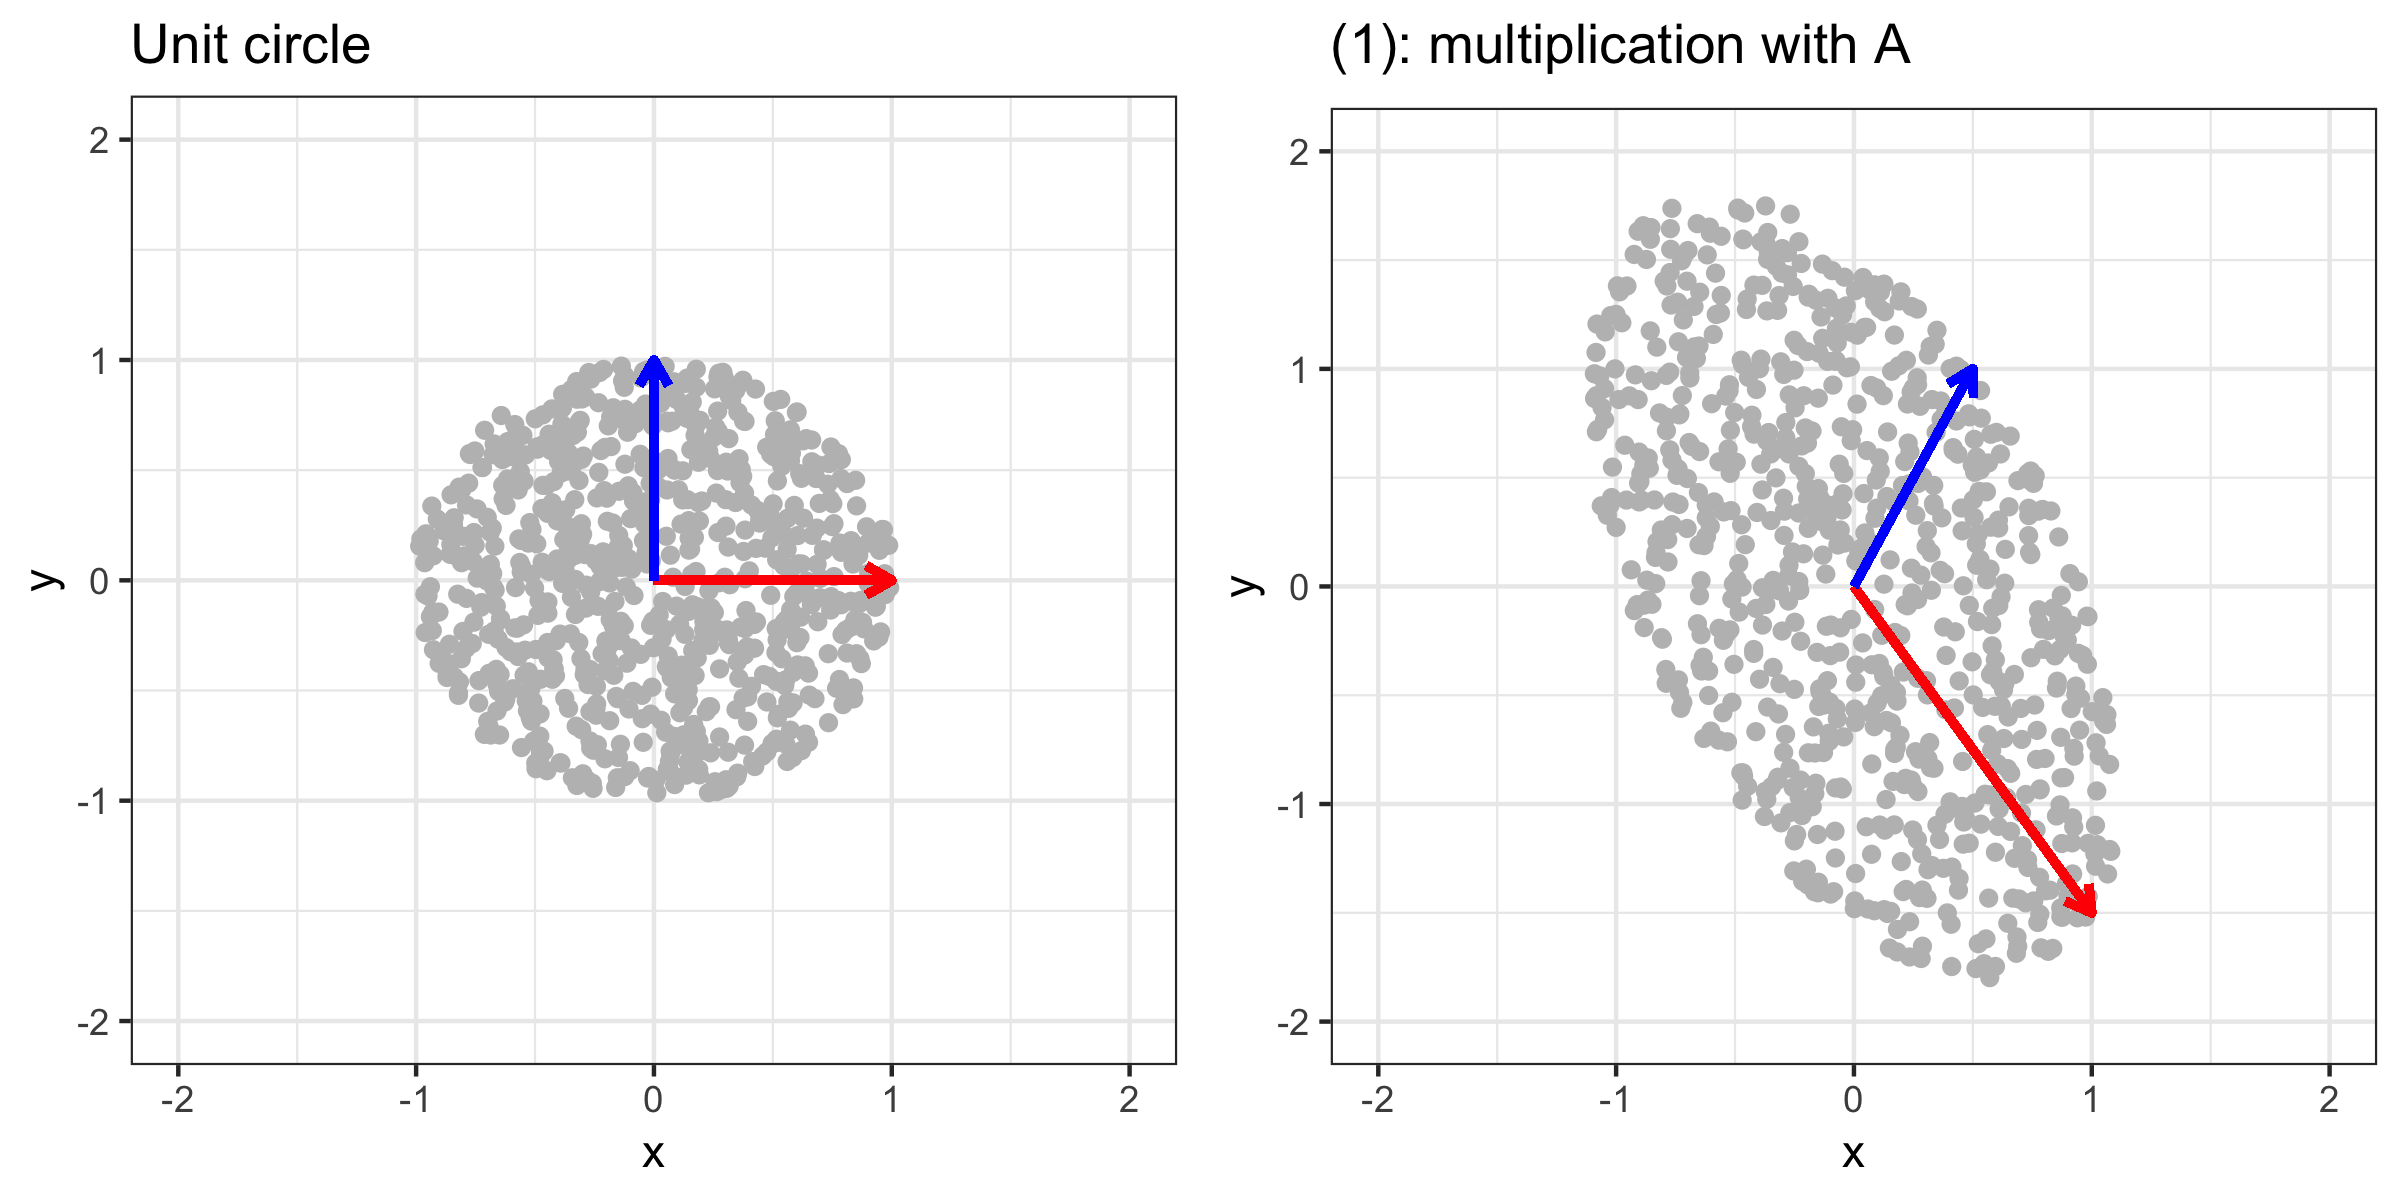
\includegraphics{figure_man/ignore/matrixabbildung.png}
\end{center}

\framebreak

It can be decomposed using the singular value decomposition:

\vspace*{1.5cm}
\begin{center}
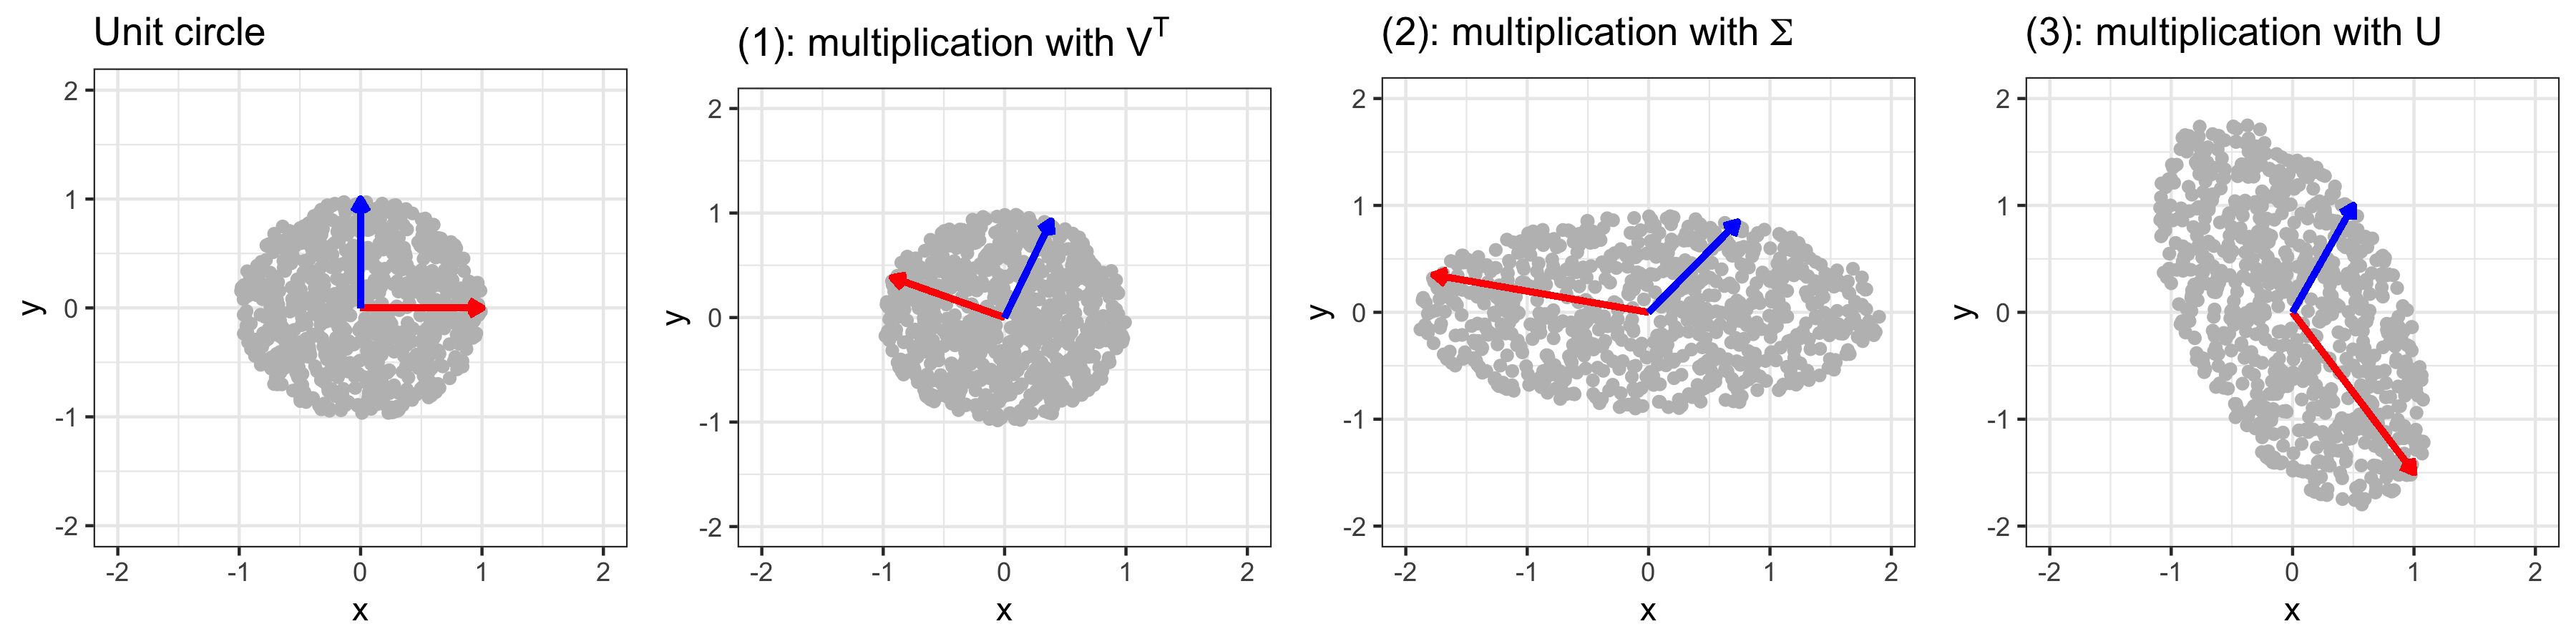
\includegraphics{figure_man/ignore/svd.png}
\end{center}

\vfill

\begin{footnotesize}
\textbf{Note:} The red / blue vectors are the canonical unit vectors $\textcolor{red}{(1, 0)^\top}$ and $\textcolor{blue}{(0, 1)^\top}$ and their transformations after the respective matrix multiplications.
\end{footnotesize}

\end{vbframe}

\begin{vbframe}{Excursus: Principal Component Analysis}

\textbf{Given: } $n$ data points with $p$ features $^{(*)}$ each

\lz

\textbf{Goal: } Projection of the $n$ data points into a $k$-dimensional space ($k < p$) with as little information loss as possible

\lz

\textbf{Idea: }

\begin{itemize}
\item Find a linear tranformation $f: \R^p \to \R^k$, which maps each observation $\bm{x}\in \R^p$ to a $k$-dimensional point $\bm{z}$.
\item Lose as little information as possible through this dimensionality reduction.
\item As little information as possible is lost if we can reconstruct the point $\bm{z}$ as good as possible, i.e. we can use a linear function $h: \R^k \to \R^p$, such that $\xv \approx h(\bm{z})$.
\end{itemize}

\vfill

$^{(*)}$ We assume the data points are centered around $0$.

\framebreak

\begin{center}
  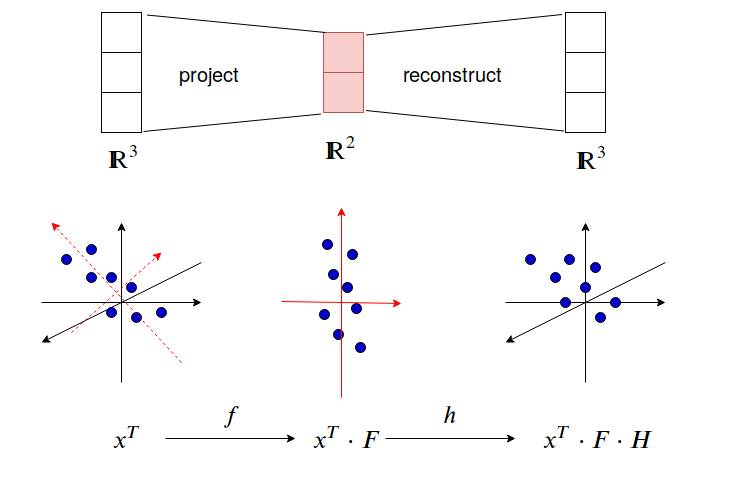
\includegraphics[width = 0.7\textwidth]{figure_man/ignore/matrixapproxi_s18.png}
\end{center}

%\vspace*{1cm}

The linear transformations $f, h$ are described by matrix multiplication: $f: \xv^\top \mapsto \xv^\top \bm{F} =: \bm{z}$ and $h: \bm{z}^\top \mapsto \bm{z}^\top \bm{H}$

\begin{footnotesize}
	Note: Here, we are writing $\xv$ as a \textbf{row vector} $\xv^\top$, to be in line with the matrix notation in the following slides (the observations are the rows of the design matrix $\bm{X}$).
\end{footnotesize}

\framebreak

\textbf{Goal:} Minimize the reconstruction error between data $\bm{X} \in \R^{n \times p}$ and the projected and reconstructed data $\bm{XFH}$.

$$
\min_{\bm{F} \in \R^{p \times k}, \bm{H} \in \R^{k \times p}} \|\bm{X} - \bm{X}\bm{F}\bm{H}\|^2_F
$$

Defining $\bm{X\bm{F}} =: \bm{W} \in \R^{n \times k}$, we write this as 

$$
\min_{\bm{W} \in \R^{n \times k}, \bm{H} \in \R^{k \times p}} \|\bm{X} - \bm{W}\bm{H}\|^2_F.
$$

This is the problem of matrix approximation. One solution is 

\begin{eqnarray*}
\bm{XF} &=&\bm{W} = \mathbf{U}_k \boldsymbol{\Sigma}_k; \quad \bm{H} =  \mathbf{V}_k^\top, 
\end{eqnarray*}

with $\bm{U}_k \in \R^{n \times k}, \boldsymbol{\Sigma}_k \in \R^{k \times k}, \bm{V}_k \in \R^{p \times k}$ chosen as truncated singular value decomposition of $\bm{X}$.

\lz 

$\bm{H} = \bm{V}_k^\top \in \R^{k \times p}$ is the reconstruction transformation matrix. The projection matrix $\bm{F} = \bm{V}_k \in \R^{p \times k}$ fulfills $\bm{XF} = \bm{U}_k \bm{\Sigma}_k$:
\begin{eqnarray*}
\bm{XF} &=& \bm{X}\bm{V}_k = \bm{U\Sigma V}^\top \bm{V}_k = \bm{U}\bm{\Sigma} \begin{pmatrix} \bm{I}_k \\ \bm{0}_{p - k}\end{pmatrix} = \bm{U} \begin{pmatrix} \bm{\Sigma}_k \\ \bm{0}_{n - k} \end{pmatrix} = \bm{U}_k \bm{\Sigma}_k,
\end{eqnarray*}

\begin{itemize}
	\item The rows of $\bm{XF} = \bm{U}_k \boldsymbol{\Sigma}_k \in \R^{n \times k}$ are the projected observations. 
	\item It can be shown (see next slide), that the rows of $\bm{H} = \bm{V}_k^\top \in \R^{k \times p}$ correspond to the $k$ (pair-wise orthogonal) principal components.
\end{itemize}

\framebreak

A more common motivation of PCA is the following: Linearly transform the data to a new coordinate system such that the greatest variance in the (transformed) data is along the first PC, the second greatest variance is along a second PC orthogonal to the first PC, etc. 

\begin{itemize}
	\item In this formulation, it can be shown that the $k$ first principal components correspond to the $k$ eigenvectors with the greatest eigenvalues of the covariance matrix $\bm{X}^\top \bm{X}$. 
	\item The eigenvalue decomposition $\bm{X}^\top \bm{X}$ and the singular value decomposition of $\bm{X}$ are related. Given the singular value decomposition of $\bm{X}$, we can derive the eingevalue decomposition of $\bm{X}^\top \bm{X}$:  
	\begin{eqnarray*}
		\bm{X}^\top \bm{X} &=& \bm{V} \boldsymbol{\Sigma} \bm{U}^\top\bm{U} \boldsymbol{\Sigma} \bm{V}^\top = \bm{V} \boldsymbol{\widehat\Sigma}^2 \bm{V}^\top
	\end{eqnarray*}
	with $\boldsymbol{\widehat\Sigma}^2 := \boldsymbol{\Sigma}^\top \boldsymbol{\Sigma} \in \R^{p \times p}$ having the squared singular values of $\bm{X}$ on the diagonal.
	\item The right singular vectors $\bm{V}$ of $\bm{X}$ are equivalent to the eigenvectors of $\bm{X}^\top \bm{X}$, and the singular values of $\bm{X}$ are equal to the square-root of the eigenvalues of $\bm{X}^\top\bm{X}$. So we come up with the same solution for both approaches. 
\end{itemize}

\end{vbframe}


\endlecture
\end{document}







